%%%%%%%%%%%%%%%%%%%%%%%%%%%%%%%%%%%%%%%%%%%%%%%%%%%%%%%%%%%%%%%
\section{Production and Assembly}
\label{sec:fdsp-pd-prod-assy}
%\metainfo{(Length: TDR=40 pages, TP=8 pages)}
%%testing
%%%%PHOTON COLLECTORS PRODUCTION %%%%%%%%%%%%%%%%%%%%%%%%%%%%%%%%%%%%%%%%%%%%%%%%%%%
The \single \dword{pds} consortium is a geographically diverse group of institutions, collaborating across three continents to fabricate a single integrated system.  As such, careful planning and control of component fabrication, assembly and testing must be maintained.

This section describes the planning for fabrication, assembly, and testing, focusing primarily on the \dword{pd} light collector modules, photosensors and photosensor modules, electronics, and calibration and monitoring.
 
%%%%%%%%%%%%%%%%%%%%%%%%%%%%%%%%%%%%%%%
\subsection{Light Collector Module Component Fabrication}

The \dword{pd} light collector modules were designed with ease of fabrication in mind.  The module components can be fabricated and \dword{qc} tested at physically separated facilities, later to be collected and assembled at one or more assembly facilities.  %Fabrication information for selected components is described below.

%%%%%%%%%%%%%%%%%%%%
\subsubsection{Dichroic filter fabrication and coating, Vikuiti reflector foils}

The baseline design for dichroic filters is 
a fused silica plate,  \SI{10}{cm}$\times$\SI{7.8}{cm}$\times$\SI{0.2}{cm}, commercially coated (as described in Section~\ref{sec:fdsp-pd-lc}) to provide for the dichroic properties of the filter.  
We plan to purchase these plates from a commercial vendor (certified by the vendor for performance), and test the performance of a representative sample at a collaboration institution.  

Prior to coating, the filters are cleaned using isopropyl alcohol according to the manufacturer's procedures. % given by the manufacturer . 
Since the most likely vector for scratching/damaging the coating is dragging contaminated wipes across the surface, new clean lint free wipes are used for each cleaning pass on the surface. Clean filters are then baked for water desorption at 100$^\circ$C for \SI{12}{hours}. 
For \dword{pdsp} \dword{pd} production the evaporation process will be performed
%at Unicamp 
in Brazil, 
%\fixme{do we want to specify institutions?} 
where a large vacuum evaporator with an internal diameter of one meter is now available. The conversion efficiency of the film deposited on the filters will be measured for a representative sample, with a dedicated set-up that will use the \SI{127}{nm} light produced by a VUV monochromator.

Vikuiti reflector foils required for the rear reflector surface of single-sided X-ARAPUCA supercells and the sides of all modules will be purchased from a vendor, laser-cut to the form factor required by the vendor prior to delivery.  Mechanical and optical \dword{qc} tests will be performed on a representative sample upon receipt.

%%%%%%%%%%%%%%%%%%%%
\subsubsection{Wavelength shifting plates}

The baseline design for the wavelength-shifting plates are %calls for a plate  composed of 
Eljen EJ-286 plates of dimensions \SI{48.7}{cm} $\times$ \SI{93.0}{cm}$\times$ \SI{0.35}{cm}.  The edges of a plate will be simultaneously cut and polished with a diamond-edged cutter to increase internal reflectivity, following a proprietary process developed by Eljen.  Plates will be delivered to the consortium institution responsible for this component, where \dword{qc} testing of a representative sample will be performed.

\subsubsection{Mechanical components}

The mechanical components of the \dword{pd} module frames is
FR-4 G-10. This material will mitigate thermal expansion issues (see thermal expansion discussion below section??), %but it imposes difficulties in the manufacturing process, as this material is abrasive and somewhat difficult and expensive to work with using traditional machining processes.
but is abrasive and somewhat difficult and expensive to work with using traditional machining processes.

To mitigate these difficulties, most of the \dwords{pd} frame components can be water-jet cut. %Most components in the design can be fabricated to completion using these techniques.  In the case where post-cutting fabrication are required, typically this is only tapping of pre-cut holes, or (rarely) drilling and tapping holes into the sides of the components where the pilot holes were not able to be pre-cut with the water jet.
In some cases post-cutting fabrication is required, e.g., tapping of pre-cut holes, or (rarely) drilling and tapping holes into the sides of the components where the water jet could not pre-cut pilot holes.

%Our plan for fabrication calls for procuring water-jet cut components from an external vendor, and conducting secondary fabrication at consortium institution(s) as required.  \dwords{qc} tests of a representative sample of finished components is planned for.
We will procure water-jet cut components from an external vendor and conduct secondary fabrication at consortium institutions as needed.  \dword{qc} tests will be conducted on a representative sample of finished components.

\label{sec:fdsp-pd-prod-pc}
%\metainfo{\color{blue} Content: Warner}

%%%%ARAPUCA %%%%%%%%
%rjw 11/20/18 No need for subsection with only one light collector!
%\subsubsection{ARAPUCA}
%\label{ssec:fdsp-pd-pc-prod-arapuca}
%\fixme{This section remains to be updated.}
% New from Ana added 8 apr 18


\subsection{Photon Detector Module Assembly}

Final assembly planning for \dword{pd} modules is guided by the assembly of \num{60} \dword{pdsp} \dword{pd} modules at the Colorado State University assembly facility. DUNE \dword{spmod} \dword{pd} module assembly will occur at one or more assembly facilities.  Our plan for distribution of the various fabrication and assembly processes to consortium institutions is still developing, as is our understanding of available resources and their optimization advances.  
%This will be resolved prior to and 
A plan will be presented at the production readiness review in fall of 2019.
%\fixme{Dave: Is this decision planned for the coming months?}
%\fixme{addressed:  DWW}
%Several features of this are common to all three types of module, and these aspects will be covered in this section.

\subsubsection{Incoming Materials Control}

All materials for \dword{pd} module assembly will be delivered with a \dword{qc} traveler (in the case of materials custom fabricated for DUNE) generated prior to arrival at the assembly site or will have an incoming materials traveler generated immediately upon receipt of the component (for commercial components).  These travelers will be scanned upon receipt at the assembly facility, and the data stored in the DUNE \dword{qc} database.  Materials will either arrive with a pre-existing DUNE inventory control batch/lot number, or will have one assigned prior to entering the assembly area.  Bar code labels attached to storage containers for all components in the assembly area will facilitate traceability throughout the assembly process.

Immediately upon receipt, all materials will undergo an incoming-materials inspection, including confirmation of key dimensional tolerances as specified on their incoming materials documentation. % for that component.  
The results of these inspections will be included on the traveler for that batch/lot and entered into the database.

In the case of a discrepancy, the deviation from nominal will be recorded in an exception section of the traveler, as will the resolution of the discrepancy.

\subsubsection{Assembly Area Requirements}

Assembly will occur in a class \num{100000} or better clean assembly area.  

%The requirement for light exposure is specified in %Table~\ref{tab:spec:env-light-exposure}.
%Table~\ref{tab:specs:SP-PDS-3}.
%\begin{table}[htp]
  \caption{Specification for SP-PDS-3 \fixmehl{ref \texttt{tab:spec:env-light-exposure}}}
  \centering
  \begin{tabular}{p{0.2\textwidth}p{0.75\textwidth}} 
     \rowcolor{dunesky}
    \newtag{SP-PDS-3}{ spec:env-light-exposure } 
                & Name: Environmental light exposure    \\ 
    Description & Blue/UV Light exposure to the PD modules should be minimized.  No exposure to sunlight at any time.  UV-Filtered light (>\SI{400}{nm}) during all exposure.   \\  \colhline
    Specification (Goal) &  \num{0} sunlight; ALARA other sources  ({ ALARA } ) \\   \colhline
    
    Rationale &  { WLS-coated filters and reflective surfaces are destroyed by prolonged exposure to light <400nm for extended periods.  Filtering is critical. } \\ \colhline
    Validation &{ Need text here. } \\    
   \colhline
  \end{tabular}
  \label{tab:spec:env-light-exposure}
\end{table}

Photosensitive components (e.g., \dword{tpb}-coated surfaces) are sensitive to near-UV light exposure, and will be protected by blue-filtered light in the assembly area (>\SI{400}{nm} or better filters\footnote{For example, GAMTUBE T1510\texttrademark{} from GAM Products, Inc., \url{http://www.gamonline.com/catalog/gamtube/index.php}.}); it has been determined that this level of filtering is sufficient to protect coated surfaces during  exposures of up to several days. For exposures of weeks or months, such as in the ProtoDUNE cryostat assembly area, a higher cutoff yellow filter is used\footnote{F007-010\texttrademark{} Amber with Adhesive - http://www.epakelectronics.com/uv\_filter\_materials\_flexible.htm.}. 


% 4/12/18 per Dave reporting on Stu's studies?
\fixme{spec table ref <--not sure what you want here Anne, we reference the relevant spec with in the table is there a better way to do it?}
Exposure of photosensitive components will be strictly controlled, per requirement SP-PDS-3 in Table~\ref{tab:specs:SP-PDS}.  
Work flow restrictions will %be restricted to 
ensure no component exceeds a total exposure of \SI{8}{hours} to filtered assembly area lighting (including testing time).

\subsubsection{Component Cleaning}

All components will be cleaned % as appropriate, 
following manufacturer's specifications and DUNE materials test stand recommendations.  %Cleaning procedures will be written for all incoming materials, and completion of these procedures noted in the appropriate travelers.
All incoming materials will have written cleaning procedures and their travelers will document the completion of these procedures.

Tests of cryogenic coating performance have demonstrated that particular care is required for the pre-cleaning of dichroic filters.  Prior to coating, the filters are cleaned per manufacturer's instructions %according to the procedures given by the manufacturer 
using isopropyl alcohol. Since the most likely vector for scratching or damaging the coating is dragging contaminated wipes across the surface, a new %clean 
lint-free wipe is used for each  cleaning pass on the surface. Clean filters are then baked at 100$^\circ$C for \SI{12}{hours} to remove water. 
%\fixme{say why}

\subsubsection{Assembly Procedures}

%Following the example of the \dword{pdsp} experience, 
As was done for \dword{pdsp}, detailed, step-by-step written procedure documents will %be followed 
guide the assembly for each \dword{pd} module, with a \dword{qc} traveler% for each module is 
completed and recorded in the database.  \dword{pdsp} experience suggests that a two-person assembly team is necessary. % for module assembly. 
%and sufficient for all three currently-considered versions of the light collector modules.  
Our current assembly plan envisions a pair of two-person assembly teams working simultaneously, %operating at the same time, 
with a fifth person acting as shift leader.  The shift leader %is not directly involved in assembly, but rather 
acts as a \dword{qc} officer responsible primarily for ensuring the distribution of materials to the assembly teams, documenting the batch and lot numbers for each \dword{pd} on the %relevant module 
travelers, and ensuring that the teams follow the documented assembly procedures. % are followed.

Assembly fixtures mounted to \SI{2.4}{m} long flat tables will %be used to 
support and align \dword{pd} components during assembly.  All workers handling \dword{pd} components will wear gloves, hair nets, shoe covers, and clean-room disposable lab jackets at all times.

\subsubsection{Post-Assembly Quality Control}

Post-assembly \dword{qc} planning is currently based on \dword{pdsp} experience, modified as appropriate for larger-scale production.  Each \dword{pd} module goes through a series of ``go-no go'' gauges 
%\fixme{go-no??} - standard terminology
designed to control tolerances of critical interface points.  Following this, each module is inserted into a test \dword{apa} support model, representing the tightest slot allowed by \dword{apa} mechanical tolerances. %Next, each module is 
It is then scanned at a fixed set of positions 
%\fixme{(to be determined prior to the TDR)} 
with \SI{275}{nm} UV \dwords{led}.  The \dword{pd}  response at each position is read out using \dword{pd} readout electronics, and the data compared to pre-established criteria.  Figure~\ref{fig:pds-pd-scanner} shows %is a photograph of 
the scanner used for \dword{pdsp} modules. These performance data will serve as a baseline for the \dword{pd} module, and will be compared against those taken in an identical scanner shortly before installation into an \dword{apa} in the \dword{spmod}, as for \dword{pdsp}. % experience.  
All data collected are recorded to the module traveler and to the DUNE \dword{qc} database.
Post-assembly immersion into a LN2 cryostat followed by a repeat scan of each \dword{pd} module (as in \dword{pdsp}) is under consideration as a final \dword{qc} check.

\begin{dunefigure}[\dword{pd} module scanner.]{fig:pds-pd-scanner}
{\dword{pd} module scanner.}
  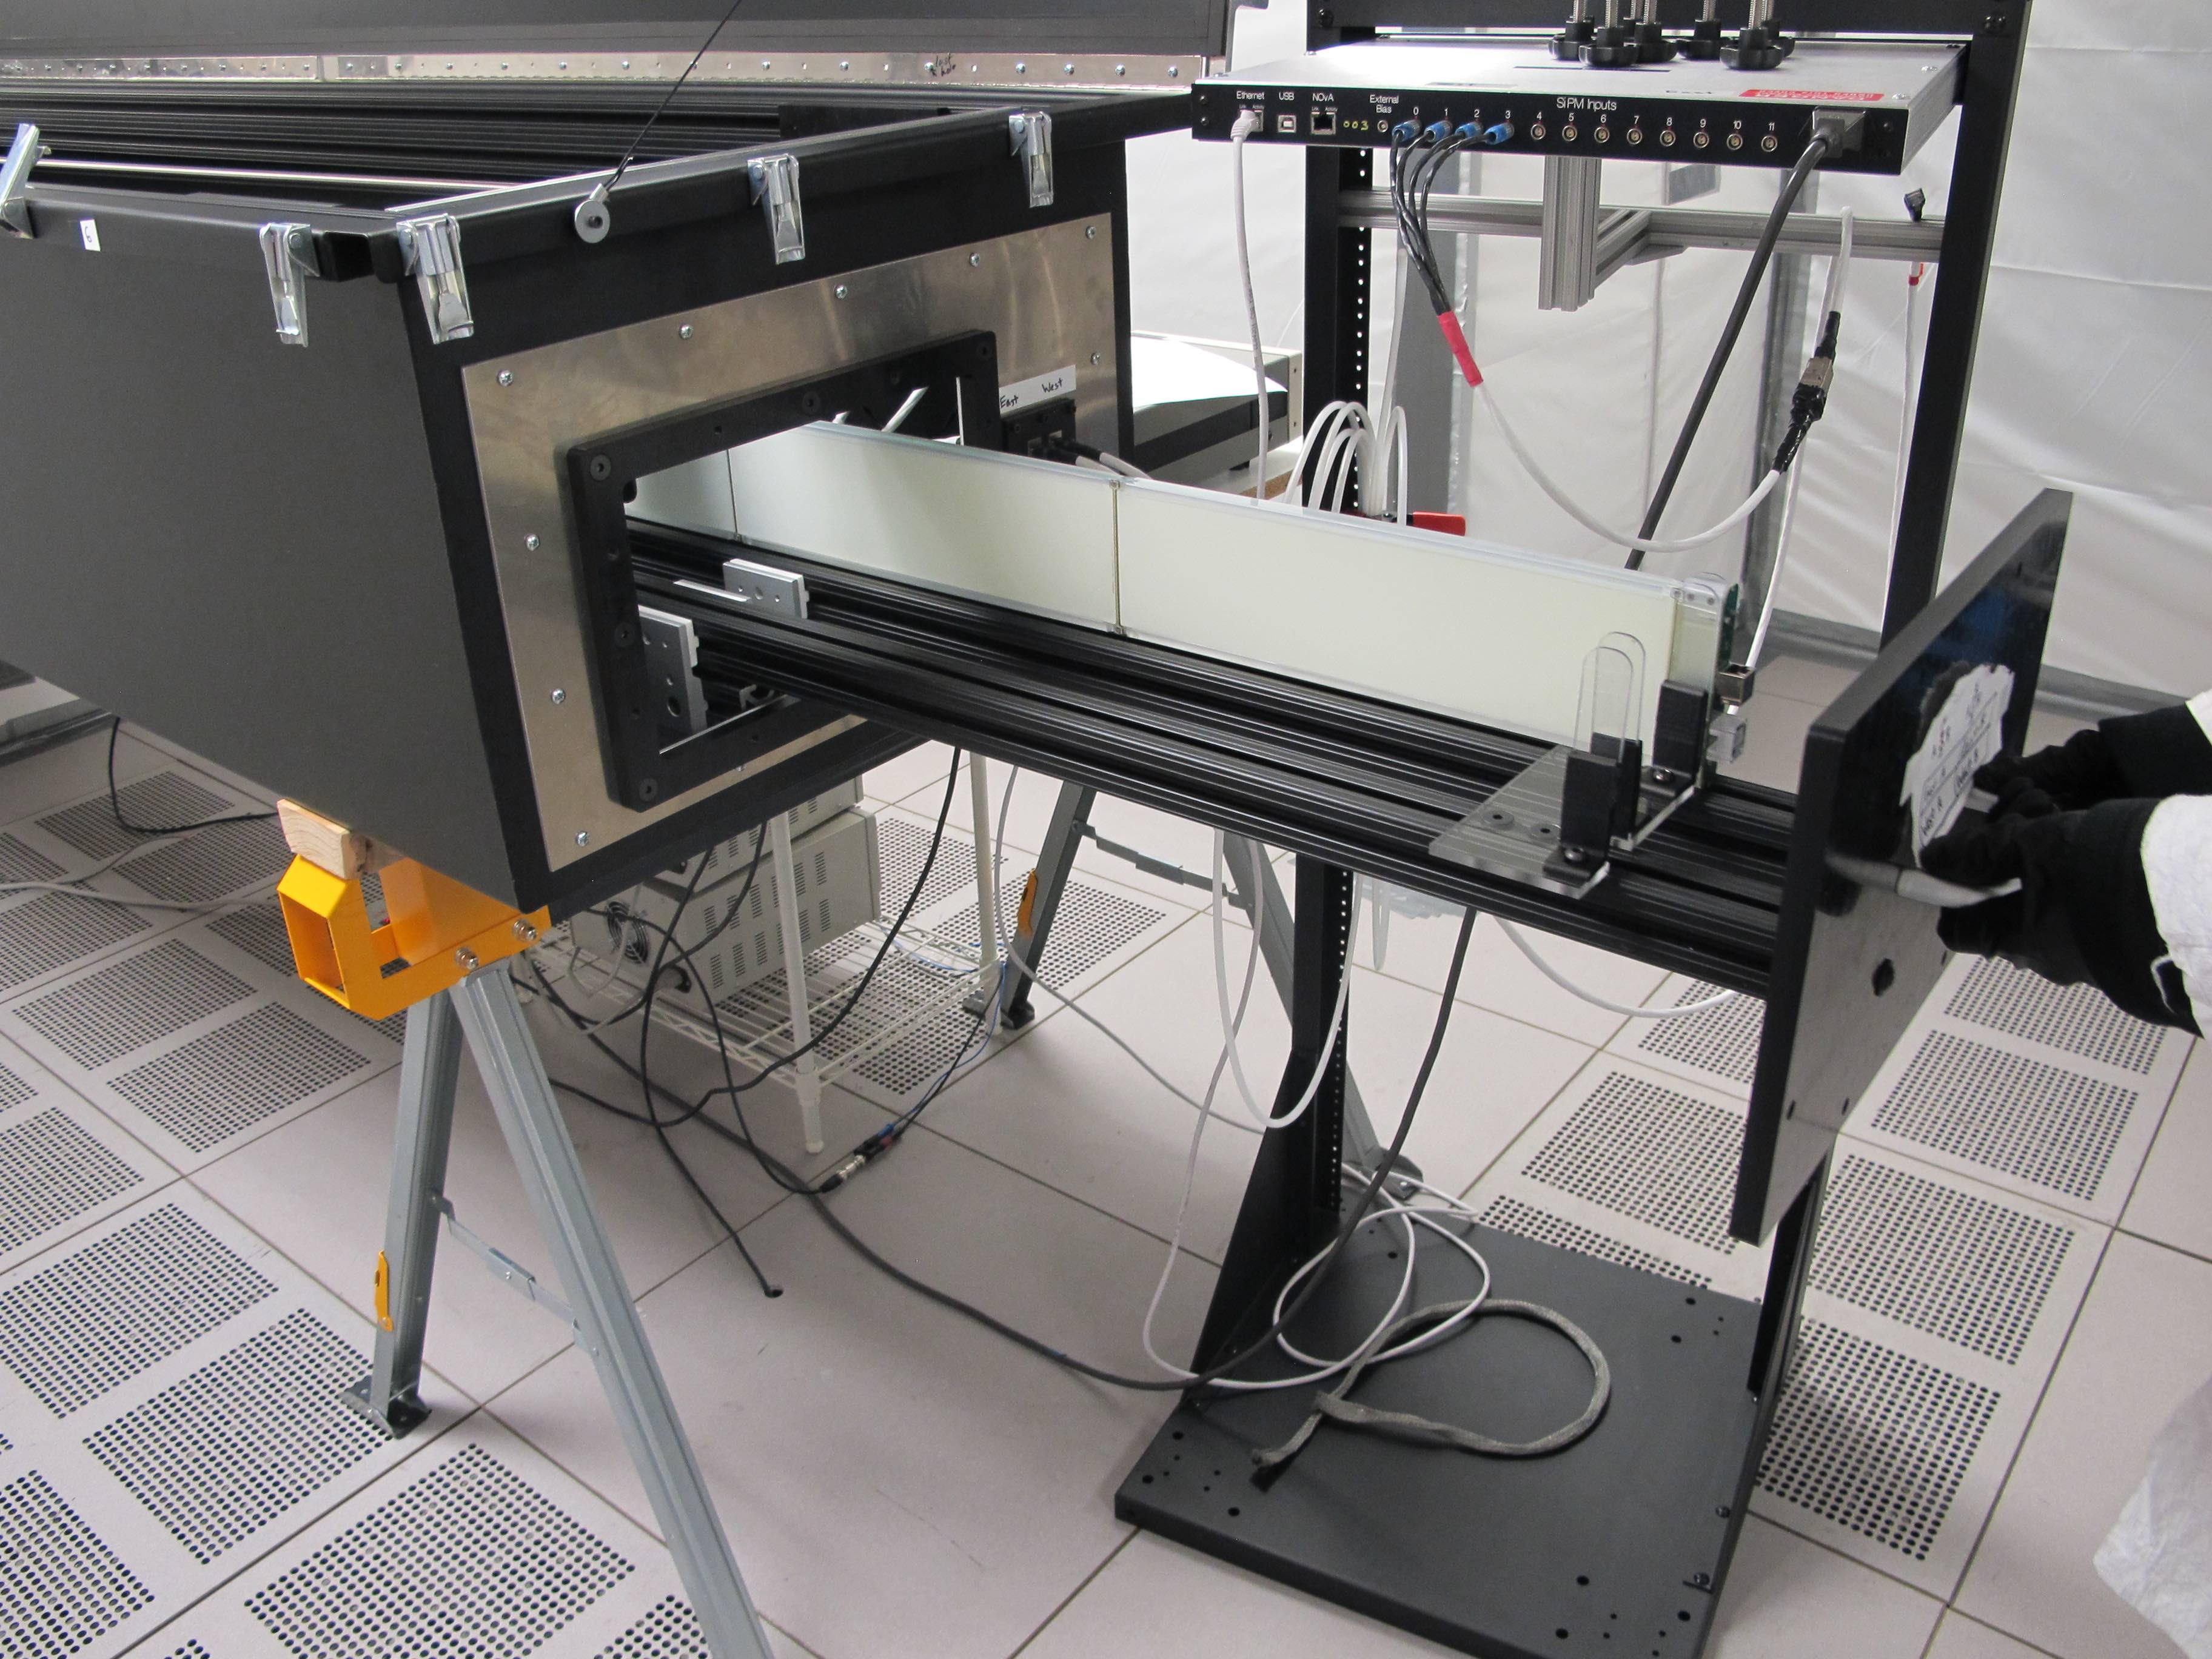
\includegraphics[width=0.5\columnwidth]{pds-pd-scanner.jpg}
\end{dunefigure}


